\subsection{Architektur}
Beim NanoPi Neo handelt es sich, wie bereits erwähnt, um einen Prozessor mit vier Kernen. Dadurch hat man die Möglichkeit vier Prozesse parallel ablaufen zu lassen. Aus diesem Grund wurde in der untenstehenden Abbildung (\fref{bArchitektur}) der Kern symbolisch in vier Abschnitte geteilt, welche die einzelnen Prozesse symbolisieren sollen. Nachfolgend werden die Aufgaben der einzelnen Kerne gezeigt, die schlussendlich das gleichzeitige Aufnehmen und Verarbeiten der Verkehrsteilnehmer ermöglichen.

\begin{figure}[H]
  \centering
  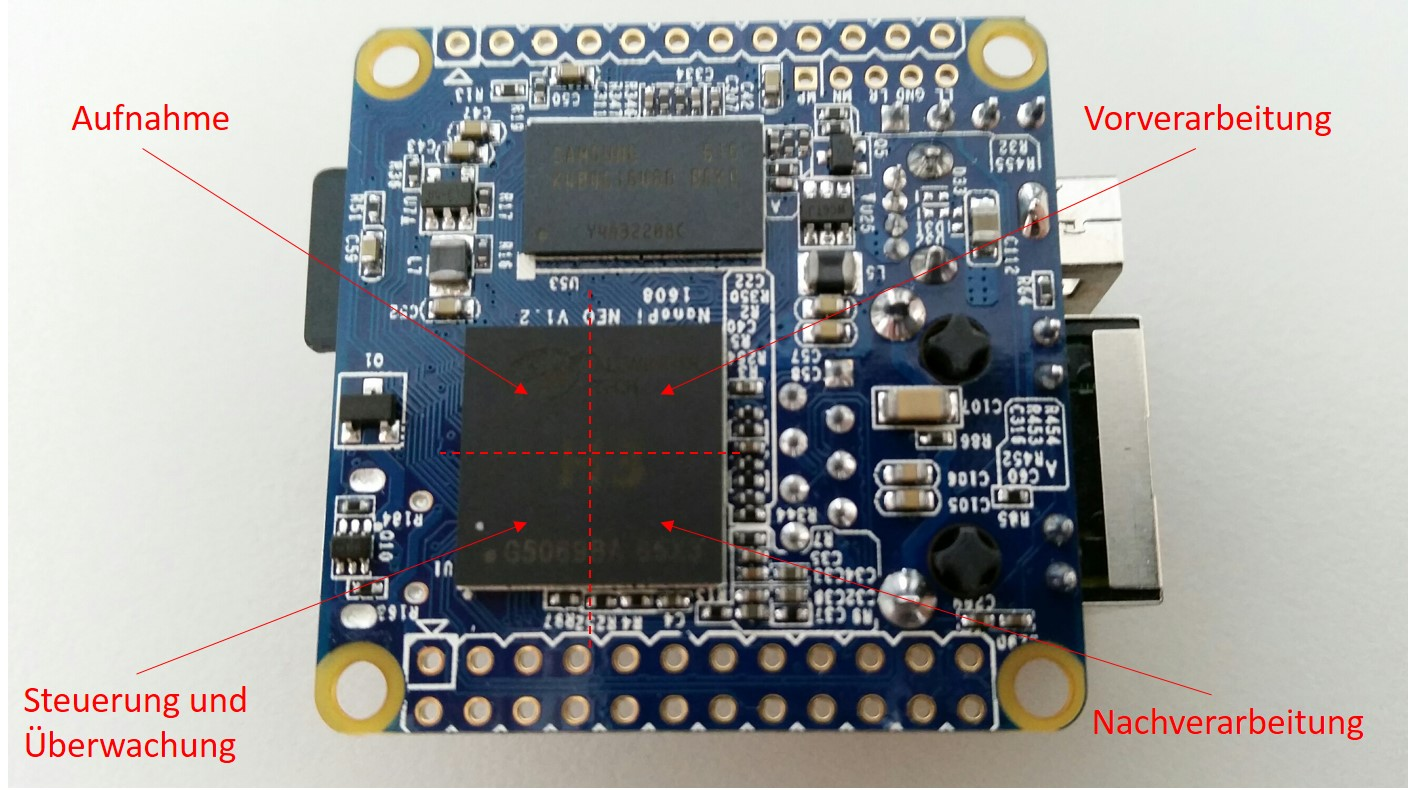
\includegraphics[width=0.99\textwidth]{Software/Architektur.jpg} 
  \caption{Aufteilung der vier Kerne.}
  \label{bArchitektur}
\end{figure}


\subsubsection{Aufnahme}
Der erste Prozess beinhaltet die Aufnahme von Videos mit der Kamera. Die Videos werden mit 25 Bildern pro Sekunde und einer Auflösung von 640x480 Pixeln aufgenommen und auf der Speicherkarte abgelegt. Dabei muss ein Video immer eine Länge von 15 Minuten erzielen, bevor es abgespeichert wird. Die Zeitspanne von 15 Minuten wurde gewählt, damit nach Abschluss dieser Zeit der nächste Prozess sich schon um die Verarbeitung kümmern kann.  Währenddessen kann sich der Aufnahmeprozess bereits mit dem nächsten Video beschäftigen. So erreicht man die parallelen Abläufe. Eine geringere Aufnahmezeit würde einen grösseren Fehler verursachen, da jedes abspeichern und neustarten eines Videos ein bis zwei Sekunden dauert, in welcher die Verkehrsteilnehmer nicht erkannt werden können. Die Videos sind im "'AVI"' Format abgespeichert und beinhalten im Durchschnitt etwa 22'500 Einzelbilder, welche dann vom nachfolgenden Prozess analysiert werden müssen. Mithilfe von Avconv werden diese Videos aufgenommen und mittels Zeitstempel, welcher Datum und Uhrzeit des Aufnahmestarts beinhaltet, im zugehörigen Ordner abgespeichert. Der Zeitstempel wird benötigt um später den Zeitpunkt eines vorbeifahrenden Verkehrsteilnehmers zu errechnen und um zu wissen, welche Videos der Reihe nach weiterverarbeitet werden müssen. Der Prozess der Videoaufnahme ist spezifisch auf den ersten der vier Prozessoren zugeteilt. Während der Aufnahmephase befindet sich dieser Kern stetig bei einer Auslastung von 95 - 100\%.

\subsubsection{Vorverarbeitung}
Sobald sich zwei Videos im dafür vorgesehenen Ordner befinden, kann davon ausgegangen werden, dass die Aufnahme des ersten Videos abgeschlossen ist. Zu diesem Zeitpunkt beginnt die Vorverarbeitung damit, die Bilder zu analysieren und diese, sobald eine Bewegung auf dem Bild erkannt wurde, in einen separaten Ordner abzuspeichern, welcher extra für diese Frames genutzt wird. Da die Videoaufnahme innerhalb von 15 Minuten jeweils 22'500 Bilder erzeugt, muss die Vorverarbeitung etwa gleich viel Bilder in der selben Zeit auswerten können. Aus diesem Grund wurde das Programm für diesen Prozess soweit optimiert, dass nur sehr wenig einzelne Schritte durchgeführt werden müssen. Diese Analyse wird mithilfe der Bildverarbeitungsbibliothek OpenCV durchgeführt. Dabei kann ein Video angegeben werden, woraufhin von diesem das nächste nicht genutzte Frame in einer temporären Variablen gespeichert wird. Mit diesen Variablen können im Anschluss weitere Berechnungen durchgeführt werden. Die Vorverarbeitung nimmt jeweils zwei aufeinanderfolgende Frames und subtrahiert bei diesen Bildern jedes einzelne Pixel an derselben Stelle voneinander ab. Falls es keine Bewegung beim spezifischen Pixel gab, so ergibt die Subtraktion der Pixel an dieser Stelle den Wert Null. Der Pixel erscheint auf diesem Bild dann schwarz. Falls sich jedoch Bewegungen abgespielt haben, ergibt diese Berechnung einen höheren Wert und es erscheint auf dem Bild heller bzw. farbig. Dies wird für jedes der 640x480 Pixel in einem Bild durchgeführt. Daraufhin werden im nächsten Schritt die erhaltenen Differenzen addiert. Folglich erhält man eine Zahl, welche die Gesamtsumme aller Differenzen dieser 307'200 einzelnen Pixel repräsentiert. Diese Zahl ist schlussendlich ausschlaggebend für eine allfällige Bewegung zwischen diesen beiden Bildern. Die nachfolgende Abbildung (\fref{bFrames}) zeigt zwei aufeinanderfolgende Frames.

\begin{figure}[H]
  \centering
  \subfigure[Frame1]{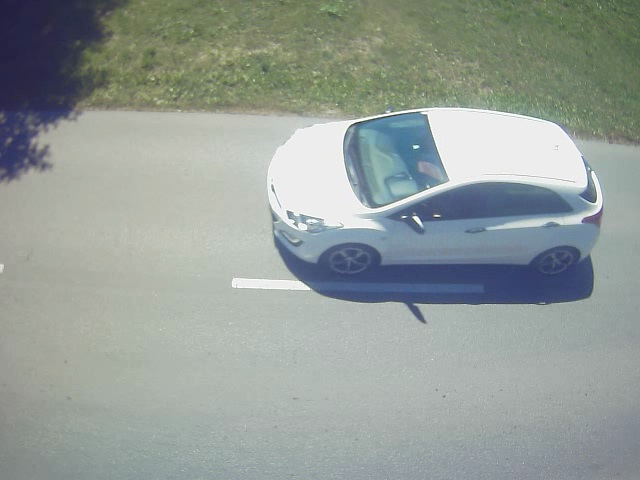
\includegraphics[width=0.49\textwidth]{Software/Frame1.jpg}}
  \subfigure[Frame2]{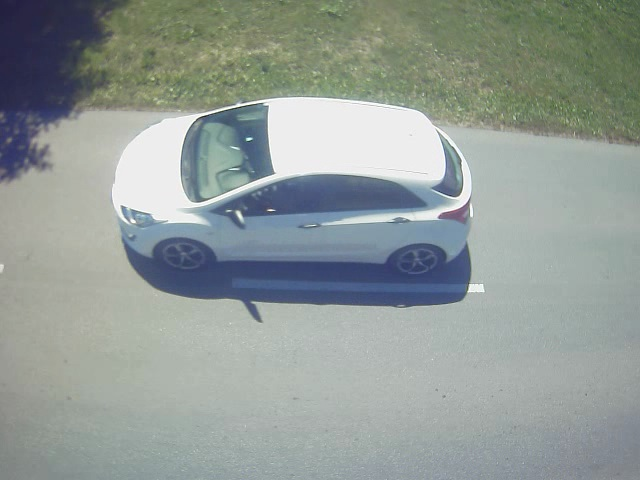
\includegraphics[width=0.49\textwidth]{Software/Frame2.jpg}}
  \caption{Zwei aufeinanderfolgende Frames.}
  \label{bFrames}
\end{figure}

Anschliessend wurde die oben erwähnte Berechnung mit diesen beiden Frames durchgeführt, wodurch Bewegungen zwischen den Bildern heller bis farbig erscheinen. Das Ergebnis der Subtraktion ist im folgenden Bild (\fref{bBlur1}) ersichtlich.

\begin{figure}[H]
  \centering
  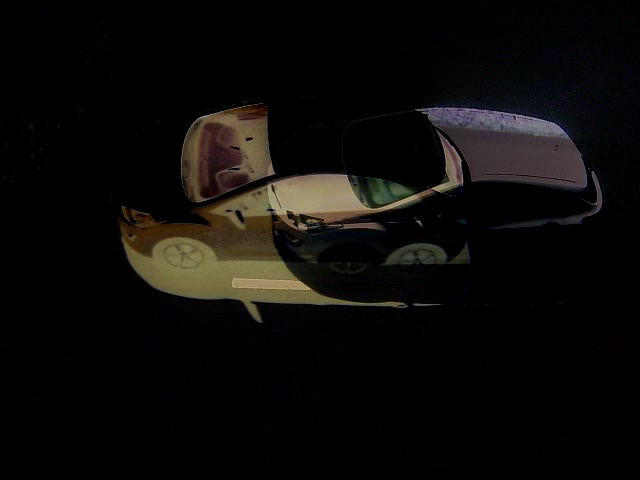
\includegraphics[height=0.3\textheight]{Software/Blur1.jpg} 
  \caption{Differenzbild der aufeinanderfolgenden Frames.}
  \label{bBlur1}
\end{figure} 

Damit ein allfälliges Rauschen oder ein vorbeilaufender Fussgänger nicht erfasst wird, wurde ein gewisser Schwellwert angegeben. Sobald die Summe der Pixel den Schwellwert überschreitet, wird das Bild temporär abgespeichert. Damit die Bilder im nächsten Schritt logisch verknüpft werden können, muss im Speichername eine Indexierung angegeben werden. Diese Indexierung ist die Zahl des Frames, welches vom Video stammt und liegt aus diesem Grund zwischen 0 und 22'499. Falls keine Speicherung stattgefunden hat wird das nächste Bild genommen und der Vorgang beginnt erneut. Mit dieser Methode werden etwa 25 Bilder pro Sekunde verarbeitet. Da jedoch für das Abspeichern der Bilder mehr Zeit benötigt wird als für das Verwerfen, können bei höherem Verkehrsaufkommen nur etwa 20 Einzelbilder verarbeitet werden. Nachdem ein komplettes Video abgearbeitet wurde, wird es aus Platzgründen und weil es für den weiteren Verlauf der Auswertung nicht mehr benötigt wird gelöscht. Dies ist die letzte Aufgabe der Vorbearbeitung. Von den 22'500 Einzelbildern, die von diesem Prozess bearbeitet wurden, sind zu diesem Zeitpunkt, je nach Verkehrsaufkommen, noch etwa 500 - 1'500 Bilder im Zwischenspeicher. Sie werden dann vom nächsten Prozess, der Nachverarbeitung, weiterbearbeitet. Da die Vorverarbeitung sehr viel Leistung erbringen muss, wurden ihm die Prozessorkerne zwei und vier zugeteilt. Die Steuerung und Überwachung, welche fix auf dem vierten Prozessorkern liegt, benötigt nur eine geringe Auslastung. Aufgrund dessen kann der Prozess der Vorverarbeitung die zwei Kerne beinahe voll auslasten, um somit die vielen Einzelbilder möglichst effizient verarbeiten zu können.

\subsubsection{Nachverarbeitung}
Nachdem die Vorverarbeitung ein Video analysiert und die relevanten Frames abgespeichert hat, kann die Nachverarbeitung beginnen. Auch hier wird der Prozess erst gestartet, wenn sich zwei unterschiedliche Ordner mit Frames im zugehörigen Ordner befinden. Somit soll gewährleistet sein, dass die Vorverarbeitung mit dem Video fertig ist, bevor die Nachverarbeitung mit dem Prozess beginnt. Das Endprodukt der Nachbearbeitung ist ein Feature Vektor. Dies ist eine Tabelle mit je einem Eintrag pro Verkehrsteilnehmer, welche mithilfe eines Tabellenkalkulationsprogramm geöffnet und bearbeitet werden kann. Dabei werden möglichst viele Indikatoren pro Verkehrsteilnehmer aufgenommen und abgespeichert. Je mehr Features pro Fahrzeug gefunden werden können, desto besser kann dieses später wiedererkannt werden und die eigentliche Verkehrsverfolgung durchgeführt werden. Nachfolgende Tabelle (\tref{tFeatureVektor}) zeigt ein Beispiel eines Feature Vektors.

\setlength\tabcolsep{5pt}

\begin{table}[H]
\centering
\begin{tabular}{|l|l|l|l|l|l|l|l|l|l|l|l|}
\hline
\textbf{I} & \textbf{Timestamp}  & \textbf{RP} & \textbf{D} & \textbf{DC} & \textbf{CropN} & \textbf{BlurN} & \textbf{PicN} & \textbf{RX} & \textbf{RY} & \textbf{RW} & \textbf{RH} \\ \hline
1            & 18.06.17 22:55:12 & 5           & R            & 1           & crop001.tif       & blur001.tif       & pic001.tif       & 95          & 141         & 377         & 190         \\ \hline
2            & 18.06.17 22:57:19 & 8           & R            & 2           & crop002.tif       & blur002.tif       & pic002.tif       & 146         & 118         & 387         & 196         \\ \hline
3            & 18.06.17 22:57:37 & 7          & L            & 1           & crop003.tif       & blur003.tif       & pic003.tif       & 138         & 145         & 373         & 251         \\ \hline
4            & 18.06.17 22:58:10 & 7           & R            & 3           & crop004.tif       & blur004.tif       & pic004.tif       & 152         & 112         & 345         & 165         \\ \hline
5            & 18.06.17 22:59:02 & 6           & L            & 2           & crop005.tif       & blur005.tif       & pic005.tif       & 115         & 126         & 415         & 296         \\ \hline
6            & 18.06.17 22:59:23 & 5           & R            & 4           & crop006.tif       & blur006.tif       & pic006.tif       & 145         & 126         & 364         & 194         \\ \hline
7            & 18.06.17 22:59:56 & 5          & R            & 5           & crop007.tif       & blur007.tif       & pic007.tif       & 113         & 100         & 453         & 311         \\ \hline
8            & 18.06.17 22:59:59 & 9           & R            & 6           & crop008.tif       & blur008.tif       & pic008.tif       & 165         & 138         & 358         & 182         \\ \hline
9            & 18.06.17 23:00:09 & 9           & L            & 3           & crop009.tif       & blur009.tif       & pic009.tif       & 148         & 160         & 367         & 212         \\ \hline
10           & 18.06.17 23:00:18 & 7           & R            & 7           & crop010.tif       & blur010.tif       & pic010.tif       & 147         & 127         & 371         & 198         \\ \hline
11           & 18.06.17 23:00:37 & 4           & R            & 8           & crop011.tif       & blur011.tif       & pic011.tif       & 155         & 128         & 341         & 189         \\ \hline
\end{tabular}
\caption{Feature Vektor.}
\label{tFeatureVektor}
\end{table}

\setlength\tabcolsep{0pt}

Der Feature Vektor zeigt den Index anhand einer fortlaufenden Nummer und den Zeitstempel, an welchem sich der Verkehrsteilnehmer in etwa in der Mitte des Kamerabildes befand. Ebenso enthält er die Information wie viele aufeinanderfolgende Bilder zu diesem Ergebnis geführt haben, in welche Richtung der entsprechende Verkehrsteilnehmer unterwegs war und einen Zähler der sowohl für links- als auch rechtsfahrende Fahrzeuge stetig erhöht wird. Daneben werden im Moment noch drei Bilder abgespeichert, welche für weitere Berechnungen von Features benützt werden können. Die letzten vier Spalten zeigen die Position des Verkehrsteilnehmers im Originalbild.\\\\
Die Nachverarbeitung kümmert sich in erster Linie darum, den Feature Vektor zu öffnen, falls dieser vorhanden ist, um daraus relevante Informationen zu entnehmen. Ist der Feature Vektor nicht vorhanden, so wird ein neuer generiert. Zu den relevanten Informationen gehört ein Index. Dieser ist notwendig, damit im Feature Vektor kein Index doppelt vorkommt und somit bereits vorhandene Bilder überschrieben werden. Zudem wird die Anzahl an Verkehrsteilnehmer, welche bis zu diesem Zeitpunkt nach links bzw. rechts gefahren sind, in einer Variablen gespeichert. Diese beiden Zähler können weiter erhöht werden, wenn neue Verkehrsteilnehmer erkannt werden. Dies ist erforderlich, da sich dieses Programm nach Abarbeitung der Frames beendet und somit alle bestehenden Informationen verliert. Anschliessend wird die Anzahl der relevanten Bilder ermittelt, welche zu einem Verkehrsteilnehmer gehören. Dies passiert, indem die Frames genommen und deren Indexierungen betrachtet werden. Falls die Indexierungen der Frames fortlaufend sind, so muss es sich zwangsläufig um denselben Verkehrsteilnehmer handeln. Falls der Abstand zwischen zwei Frames einen gewissen Wert überschreitet, hat die Kamera für kurze Zeit keine Bewegung erkannt. Folglich muss es sich dann um einen neuen Verkehrsteilnehmer handeln. Sobald die Zahl der relevanten Bilder bekannt ist, werden diese logisch miteinander verknüpft.\\\\
Aus diesen etwa drei bis zehn Bildern, je nach Geschwindigkeit des Fahrzeugs, wird nun mit der Bildverarbeitungsbibliothek OpenCV ein "'Blob Detection"' mit anschliessendem "'Blob Tracking"' durchgeführt. Zuerst werden Bewegungen zwischen zwei aufeinanderfolgenden Bildern ermittelt und dann um die Pixel in der unmittelbaren Umgebung eine konvexe Hülle, die auch Blob genannt wird, gebildet. Auf den fortlaufenden Bildern wird sich diese konvexe Hülle immer weiter zum Rand bewegen. Im Programm selbst wurde festgelegt, welche Voraussetzungen erfüllt werden müssen, damit dieser Blob als Verkehrsteilnehmer gezählt wird. Dazu gehören die Fläche der Hülle, das Verhältnis zwischen Länge und Breite, die minimale Breite und Länge und die minimale Länge der Diagonale. Falls es sich beim Blob um einen Verkehrsteilnehmer handelt, muss noch ermittelt werden, zu welchem Zeitpunkt dieser die Mitte passiert und somit die Bilder generiert werden müssen. Dies wird mithilfe einer imaginären Linie durchgeführt, welche sich in der Mitte des Bildes befindet. Da die Position des Blobs von Anfang an bekannt ist, kann auch ermittelt werden, ob der Verkehrsteilnehmer von links nach rechts oder von rechts nach links gefahren ist.\\\\
In nachfolgender Abbildung (\fref{bMotionDetection}) ist ein von rechts nach links fahrendes Fahrzeug dargestellt, welches von der Kamera erfasst wurde. Dabei wurde das Fahrzeug auf drei Frames als Ganzes abgebildet. Da dieses Auto alle festgelegten Parameter erfüllt, wird es als Verkehrsteilnehmer erkannt und eine konvexe Hülle gebildet. Die konvexe Hülle wird immer um zwei nachfolgende Frames gebildet, weshalb diese bei sämtlichen Bildern länger als der entsprechende Verkehrsteilnehmer ist. Im ersten und zweiten Frame befindet sich die Mitte der konvexen Hülle und damit auch die Mitte des gelben Quadrats jeweils auf der rechten Seite der Linie. Zu diesem Zeitpunkt wurde noch keine Zählung durchgeführt. Erst beim dritten Frame hat die Mitte des Blobs die rote Linie überquert. Dadurch wurde die Funktion zum Abspeichern eines Fahrzeugs und generieren einer neuen Zeile im Feature Vektor ausgelöst.

\begin{figure}[H]
\centering
	\subfigure[Blob Frame 1]{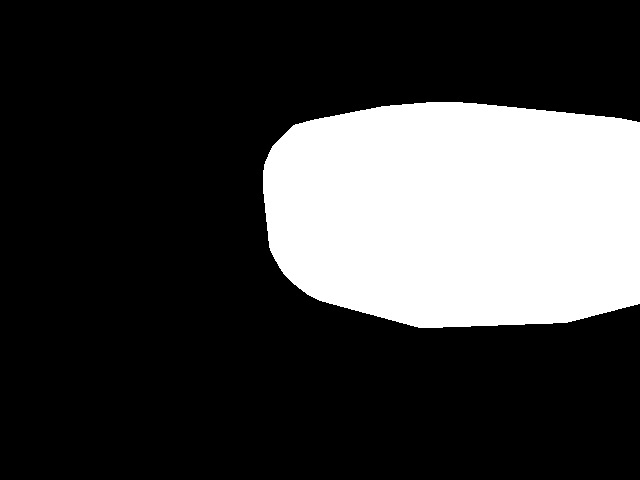
\includegraphics[width=0.48\textwidth]{Software/Blob1.jpg}}\quad
   \subfigure[Bild Frame 1]{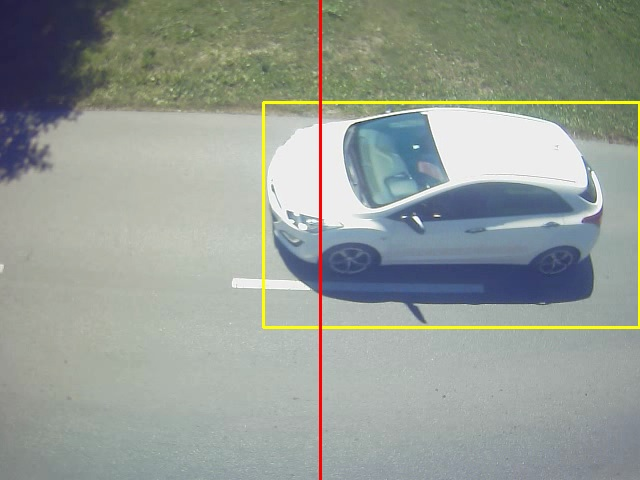
\includegraphics[width=0.48\textwidth]{Software/Detection1.jpg}}\\
   \subfigure[Blob Frame 2]{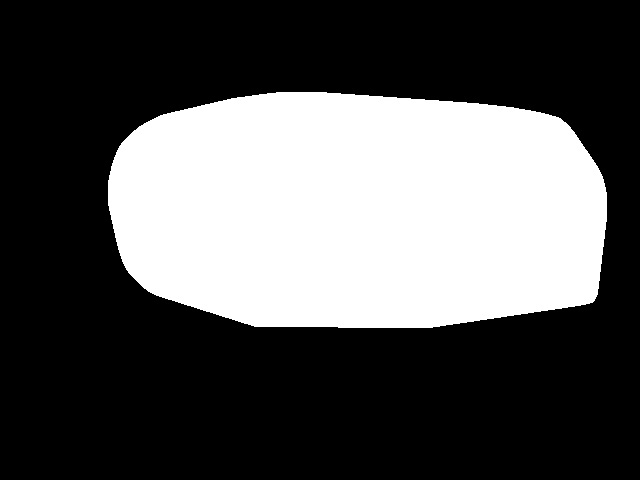
\includegraphics[width=0.48\textwidth]{Software/Blob2.jpg}}\quad
   \subfigure[Bild Frame 2]{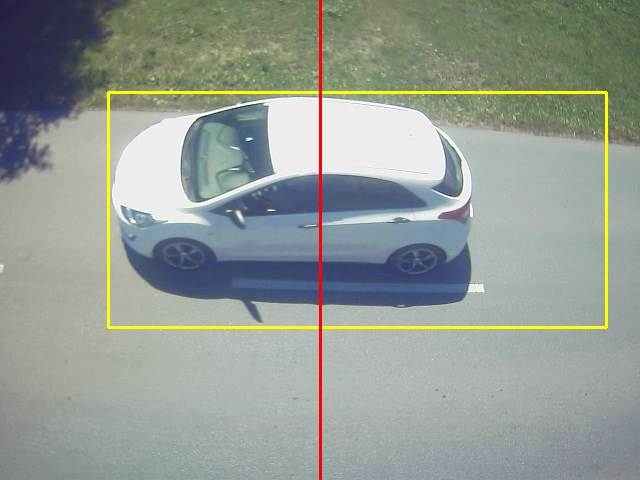
\includegraphics[width=0.48\textwidth]{Software/Detection2.jpg}}\\
   \subfigure[Blob Frame 3]{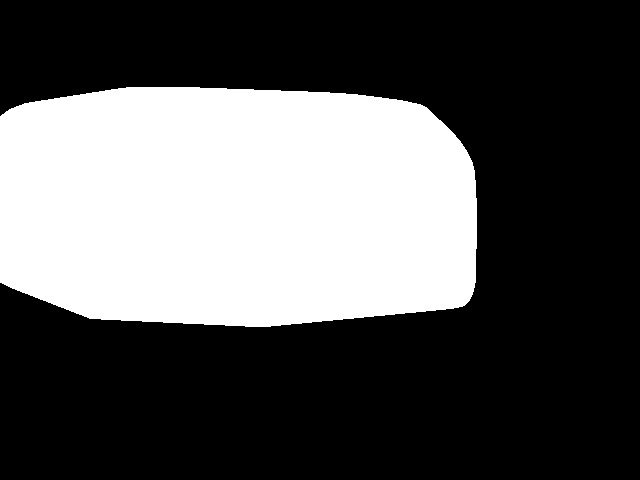
\includegraphics[width=0.48\textwidth]{Software/Blob3.jpg}}\quad
   \subfigure[Blob Frame 3]{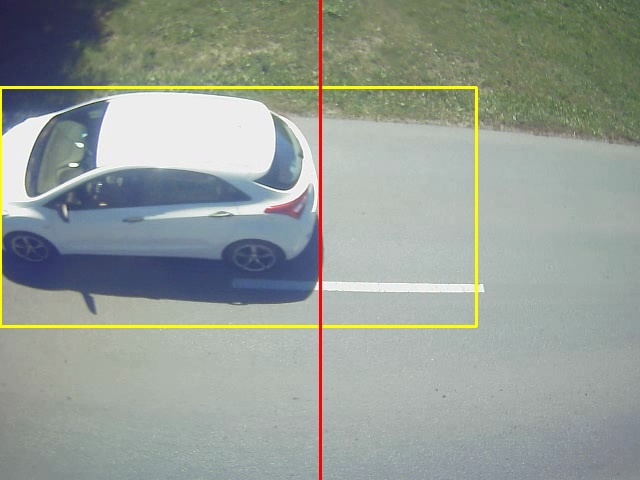
\includegraphics[width=0.48\textwidth]{Software/Detection3.jpg}}
\caption{Vehicle Tracking mithilfe von Blobs.}
\label{bMotionDetection}
\end{figure}

Die drei vorher erwähnten Bilder werden in den entsprechenden Ordnern im Speicher abgelegt und alle relevanten Informationen an den Filehandler übergeben. Dieser öffnet die Datei des Feature Vektors und schreibt alle Informationen inklusive berechnetem Zeitstempel in eine neue Zeile. \\\\
Nach diesem Vorgang ist der Verkehrsteilnehmer erfolgreich aufgenommen und abgeschlossen. Der nächste Teilnehmer kann nun ermittelt werden.\\\\
Wenn sich keine Bilder mehr im Frames-Ordner befinden, beginnt die letzte Aufgabe dieses Programms. Der bereits bearbeitete Ordner wird gelöscht, da auch dieser für die weitere Auswertung nicht mehr benötigt wird. Der Nachbearbeitung wurde fix der dritte Prozessorkern zugeteilt. Bei hohem Verkehrsaufkommen benötigt diese auch die vollen 100\% dieses Kerns.\\\\
Diese Software basiert auf dem Grundgerüst von C. Dahms "'OpenCV\_3\_Car\_Counting\_Cpp"'-Projekt \cite{OpenCVCC} und wurde an die Aufgaben von "'Fast and Curious"' angepasst, verändert und erweitert.

\subsubsection{Steuerung und Überwachung}
Vorhin wurde bereits erwähnt, dass sich die Prozesse selber beenden, sobald sie ihre Arbeit erledigt haben. Folglich wird ein Prozess benötigt, der sich hauptsächlich um die gesamte Koordination kümmert. Videos werden nur zwischen morgens um 05:00 Uhr und abends um 21:00 Uhr aufgenommen. Dies ist notwendig um sicherstellen zu können, dass alle Videos bis zum nächsten Morgen bearbeitet wurden. Dadurch soll ein Speicherplatzproblem verhindert werden, falls die Vorverarbeitung aufgrund eines hohen Verkehrsaufkommens die Videos langsamer prozessiert als diese aufgenommen werden.\\\\
Die Steuerung und Überwachung ist so konzipiert, dass sie ständig eine Schleife von Befehlen durchläuft. Die erste Aufgabe besteht darin den aktuellen Zeitpunkt zu kontrollieren. Falls die Nachtphase noch nicht aktiv ist wird im nächsten Schritt geprüft, ob der Prozess zur Videoaufnahme noch läuft. Dadurch kann sofort ein neuer Prozess zur Aufnahme gestartet werden, falls kein Video mehr aufgenommen wird.\\\\
Als nächstes wird die Anzahl der Videos im dazugehörigen Ordner kontrolliert und anschliessend auch hier der Prozess zur Vorverarbeitung analysiert. Wenn die Vorverarbeitung nicht läuft, muss diese neu gestartet werden. Dazu wird jedoch der Pfad zum Video benötigt, welches als nächstes bearbeitet werden muss. Aus diesem Grund muss es möglich sein den Pfad anhand des Erstellungsdatums der Videos herauszulesen. Danach kann die Vorverarbeitung mit dem dazugehörigen Pfad des Videos gestartet werden.\\\\
Nach dem gleichen Konzept geht es auch beim dritten Prozess, der Nachbearbeitung, weiter. Der einzige Unterschied zwischen dem zweiten und dritten Prozess besteht darin, dass hierfür zum Starten der Pfad zum Ordner mit den Frames benötigt wird.\\\\
Da nebenbei noch ein Webserver läuft, der Informationen über das System bereitstellt, hat die Steuerung und Überwachung noch kleinere Aufgaben. Dies bedeutet, auf Eingaben der Website zu reagieren und Ordner zu erstellen oder zu verschieben, wenn dies vom Benutzer gewünscht wird. Zudem ist eine Temperaturüberwachung eingebaut. Einmal pro Minute wird die Kerntemperatur ausgelesen und in ein File geschrieben. Diesem Prozess ist der vierte Prozessorkern zugeteilt. Da die Auslastung des Scripts jedoch nicht sonderlich hoch ist, teilt sich dieser Prozess den Kern mit der Vorverarbeitung. \cite{Bash}
